\chapter{Figures and Tables} \label{chap:figuresTables}

Hier finden Sie nun Beispiele für das einfügen von Grafiken und Tabellen. Für Tabellen können Sie auch Umgebungen wie tabularx und longtable verwenden.

We performed experiments for three different product categories ranging from commodity products (energy-saving lamps) over hotel rooms to capital goods (washing machines). A lower average price of the products represents a lower perceived risk. We used energy-saving lamps as rather low priced products (avg.\ price: 7.57\euro), hotel rooms as medium priced products (avg.\ price: 249.50\euro) and washing machines as rather high priced products (avg.\ price: 524.33\euro). For each category, we collected data for 40 products. Each product is described by five attributes. Specifically, we extracted frequently used attributes from Amazon product descriptions (energy-saving lamps, washing machines) or descriptions in the hotel booking platform HRS. Table \ref{tab:productsExp1} summarizes products and product attributes\footnote{For washing machines and energy-saving lamps, consumer ratings are from Amazon; for hotel rooms, consumer ratings are from hrs.com. The attribute level order for washing machine brands is based on the brands' average sales rank on Amazon.}.

 \begin{table}[!ht]
	\caption{Products and their Attributes}\label{tab:productsExp1}
	\begin{center}\small
		\begin{tabularx}{15cm}{llll}
			\hline
			Product & Attribute & Unit & Attribute Level Order\\
			\hline
			Energy-saving & Price & Euro & Increasing \\
      Lamp& Energy Efficiency Grade & -- & A+ $\succ$ A $\succ$ B  \\
      (n=40)& Deviation from Day Light & -- & None $\succ$ Low $\succ$ Large \\
      & Durability & Hours working time & Decreasing \\
      & Customer Rating & 1-5 Stars & Decreasing \\
			\hline
			Hotel Room & Price per Night & Euro & Increasing \\
      (n=40)& Category & Stars & Decreasing \\
      & Distance from City Center & Kilometers & Increasing \\
      & WLAN availability & -- & Available $ \succ$ Not available \\
      & Customer Rating & 1-5 Stars & Decreasing \\
			\hline
			Washing & Price & Euro & Increasing \\
      Machine& Brand & -- & Siemens $\succ$ Bosch $\succ$ AEG \\
      (n=40)& & & $\succ$ Bauknecht $\succ$ Gorenje \\
      & & & $\succ$ Blomberg $\succ$ LG \\
      & Energy Consumption & kWh per year & Increasing \\
      & Water Consumption & Liters per year & Increasing \\
      & Customer Rating & 1-5 Stars & Decreasing \\
			\hline			
      \multicolumn{3}{l}{$\succ$\emph{: is preferred over}}
		\end{tabularx}
	\end{center}
\end{table}

\begin{figure}[t]
  	\caption{Example Product Domination Graph}\label{fig:productGraph}
  	\begin{center}
 		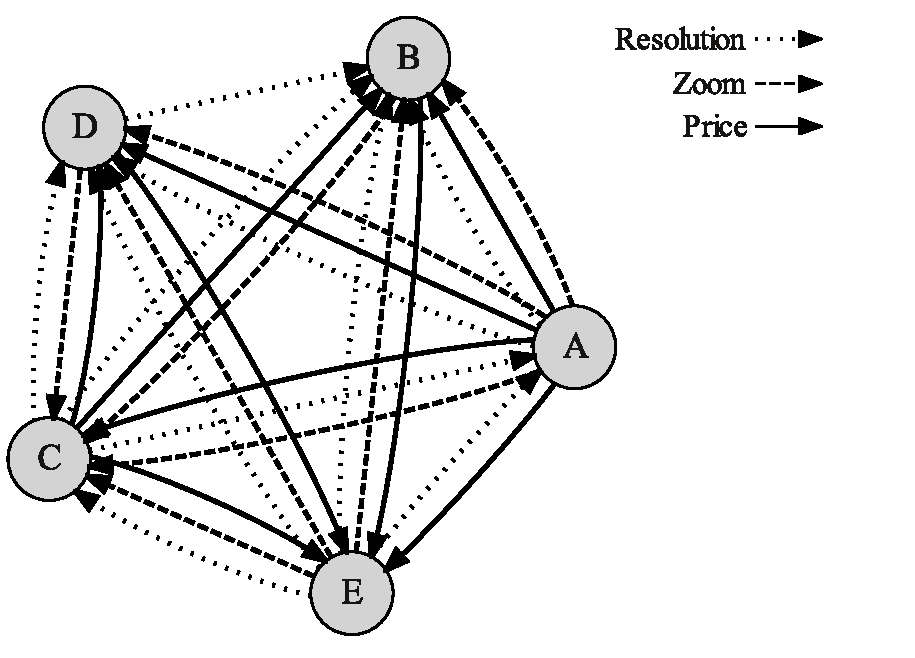
\includegraphics[width=10cm]{graphics/ProductDominationGraph}
 	\end{center}
\end{figure}

Let us give an example. We assume a choice scenario with five different cameras (see Table \ref{tab:cameras}). Product attributes are photo resolution $ph$, zoom factor $zf$, and price $pr$. All consumers have the same preference for the attribute level order: they prefer lower to higher prices, and higher photo resolutions and zoom factors to lower ones. Table \ref{tab:cameras} lists the five exemplary cameras with their corresponding attribute levels as well as single-attribute values $v_{i}$ for each attribute $a_i\in\{ph, zf, pr\}$.
Camera $E$ has the best price, but the worst photo resolution. In the product domination graph, $E$ has hence no outgoing edges with respect to price, but four outgoing edges with respect to photo resolution. Figure \ref{fig:productGraph} shows the resulting product domination graph.

Eine Tabelle finden Sie in Tabelle \ref{tab:cameras}.
\begin{table}%[!h]
	\caption{Example attribute levels and corresponding single-attribute values $v_i$}\label{tab:cameras}
	\begin{center}\small
		\begin{tabular}{lrrr}  		
			\hline
			Camera & Photo Resolution & Zoom Factor & Price\\
			\hline
			A & $v_{ph}(12 MP) = 0.60$ & $v_{zf}(10x) = 0.00$ & $v_{pr}(610 EUR) = 0.00$\\
			B & $v_{ph}(14 MP) = 1.00$ & $v_{zf}(15x) = 0.63$ & $v_{pr}(470 EUR) = 0.40$\\
			C & $v_{ph}(10 MP) = 0.20$ & $v_{zf}(18x) = 1.00$ & $v_{pr}(540 EUR) = 0.20$\\
			D & $v_{ph}(13 MP) = 0.80$ & $v_{zf}(15x) = 0.63$ & $v_{pr}(470 EUR) = 0.40$\\
			E & $v_{ph}(9 MP) = 0.00$ & $v_{zf}(10x) = 0.00$ & $v_{pr}(260 EUR) = 1.00$\\
			\hline
		\end{tabular}
	\end{center}
\end{table} 	

